\clearpage

\chapter{Mini Project 1}
\section{Digital Automata}
\horizontalline{0}{0}

\textbf{Learning Goals:}

\begin{itemize}
    \item Use metacognition skills to examine your own learning and thought processes while learning to use CoSpaces.
\end{itemize}

Whether or not you have programmed before, learning something completely new triggers an opportunity for you to examine how you approach a new problem or situation. Do you read instructions? Dive right 
in? How do you deal with a roadblock or frustration? Do you enjoy success? At what point do you know you have ‘mastered the task?’

\begin{itemize}
    \item Use basic coding commands to create a digital automata and have a shared programming experience as a course reference.
\end{itemize}

In this course we will be referencing computer programming and algorithmic tasks. This little project will give us a shared programming experience. If you are new to coding, all the basic ideas are here. 
If you are an expert, try to see how these simple blocks reflect advanced concepts.

\begin{itemize}
    \item Use a digital automata to reinforce the themes of Module One, “Mind and Machine.”
\end{itemize}

As you create your digital automata, consider how it is the same and different from mechanical automata. What features make your creation more ‘real?’ Is a mechanical automata more wondrous? How can we use 
this example to explore the idea, “mind is to brain and software is to hardware?” \vspace*{1em}

\textbf{Deliverables:}

\begin{itemize}
    \item A Cospaces activity created individually or with pairs.
    \item Mini Project Narrative - submitted and graded in Gradescope.
\end{itemize}

\textbf{Creating a CoSpace Digital Automata} \vspace*{1em}

Login to \href{https://cospaces.io/edu/}{CoSpace} with your colorado.edu account. Enter CoSpace class code given in Moodle - if needed we may open a second Cospace class. If you’d like to work with a partner 
to make a pair of interactive automata - contact your Instructor. \vspace*{1em}

\textbf{Background} \vspace*{1em}

If you have never programmed before, go to \href{https://blockly.games/}{Blockly} to try some simple code games first. \vspace*{1em}

Mechanical Automata: Watch examples of mechanical automata on youtube:

\begin{itemize}
    \item \href{https://www.youtube.com/watch?v=YAg66jrvpHA}{Video 1} (first six minutes)
    \item \href{https://www.youtube.com/watch?v=DgIDStgaybc}{Video 2}
    \item \href{https://www.youtube.com/watch?v=L3Die7PfKvo}{Video 3}
    \item \href{https://www.youtube.com/watch?v=-OJ1Yc2SwAs}{Video 4}
\end{itemize} 

Watch the CoSpace video tutorial. \vspace*{1em}

\textbf{Now Create a Digital Automata in your Cospace assignment} \vspace*{1em}

Your automata should:

\begin{itemize}
    \item Be an original creature in Cospaces (i.e. not the from the demo) in the spirit of mechanical automata.
    \item Create the action(s) of a living creature - make it seem ‘alive’ using an ‘action’ and speech.
    \item Include dialog.
    \item Include movement.
    \item Option - with a partner, create automata that interact with each other.
\end{itemize}

\textbf{Submit the narrative as PDF in Gradescope.}

\begin{itemize}
    \item For 1 - 4 the content must fit exactly on the pages given.
    \item Include these first 2 pages as is.
    \item Add as many pages as needed at the end for screenshots.
    \item Don’t forget to include your name.
\end{itemize}

% Problem 1
\begin{problem}{Problem 1}
    \begin{statement}{Problem Statement}
        Describe your Digital Automata -  What does it do?
    \end{statement}

    \begin{highlight}[Response]
        My digital automata's name is Jeremy. Jeremy is stationed on the moon and he first introduces his name and welcomes you to the moon. Upon the beginning of scene of which Jeremy is in, he tells
        the user (the person observing the scene) that he is going to ask you a series of riddles. During all of this, Jeremy is waving his hands in the air because he is so excited to have a visitor
        at his new home.

        Upon answering the first riddle, there are several choices that the user can select to the riddle. If the user answers incorrectly, Jeremy temporarily disappears and reappears after a couple of
        seconds. If the user answers the riddle correctly, then Jeremy responds with a prompt that congratulates the user for such a good answer. Regardless of the correctness of the answer, Jeremy's
        shirt changes color and he then moves to a different spot on the moon where he prepares the user for another riddle.

        After relocating to a different spot on the moon, he asks the user a different riddle. The user then has to answer the second riddle and upon answering, Jeremy responds with different ways depending
        on if the player answers correctly. After the second riddle, Jeremy's shirt changes color again and he moves to a different spot on the moon and gets stuck. After he is done moving, he recognizes
        that he is stuck and turns around to come ask the user the final riddle.

        Once the final riddle is answered, Jeremy again responds according to how the user answers the question and proceeds to do a `trick' where he moon walks, levitates, and jumps very high and comes
        back down to the surface of the moon. After all of this is done, Jeremy tells the user that they are welcome back at anytime for more fun riddles.

        My CoSpace can be found by clicking the following link: \href{https://edu.cospaces.io/YQK-GCJ}{Jeremy On The Moon}.
    \end{highlight}
\end{problem}

% Problem 2
\begin{problem}{Problem 2}
    \begin{statement}{Problem Statement}
        In 3-5 paragraphs, on this page, describe your process of learning how to use CoSpaces. What was familiar? What was challenging? How does it feel to be learning something new? How did you react 
        or deal with challenges or roadblocks?
    \end{statement}

    \begin{highlight}[Response]
        When I first started making my project in CoSpaces, it was very foreign to me and I had to watch a couple of videos describing how to actually make an environment and customize it. Upon creating a
        playground environment, I had to do a bunch of trial runs with objects to see how CoSpaces worked in the first place. This took a lot of trial and error to figure out what does what and how the settings
        worked. After getting a general idea of how you could put objects into the environment, I then dove started looking into how I could customize my objects.

        Getting my automata Jeremy to work was pretty challenging at first. I had the idea of him asking the user a series of riddles as part of the interaction with the automata but it was very difficult
        for me at the beginning to figure out how to do this. The missing link for me was that you had to enable the object that you put in the environment to be eligible to be `coded' with CoSpaces. After this,
        I started looking at the different actions that I could take to achieve the goal that I set out for me to do.

        Upon figuring out how to create something in CoSpaces, it felt really rewarding to get past my initial hurdles. I have a bunch of prior programming experience to this so the entire process felt familiar
        to learning how to use a new IDE, learning a new language, or implementing some new aspect into a program that I have been working on for some time. Getting Jeremy to do what I wanted him to do after
        struggling to do so felt reminiscent of solving a seg fault error in C++ my first time. I enjoyed the process a lot and I honestly believe that more high school should do some sort of activity with 
        CoSpaces to get kids into programming at a younger age.

        When I first was running in to roadblocks with CoSpaces, it was very frustrating. I thought to myself `There is probably some eight year old kid who figured out how to use this thing faster than I did'.
        I had to implore my typical technique of learning something new and just clicking every option that was available and seeing how it affected what I was working on. After some time, I was able to deduce
        what it was that I was doing wrong and it gave me a clearer outlook on what I needed to research in order to solve the problem that I was having. I can see how CoSpaces would be a very good introductory
        tool to people who have never programmed before, it is a great way to get people to start thinking how to make something with a computer.
    \end{highlight}
\end{problem}

% Problem 3
\begin{problem}{Problem 3}
    \begin{statement}{Problem Statement}
        In 3-5 paragraphs, describe your programming experience and how it relates to using drag and drop code.
    \end{statement}

    \begin{highlight}[Response]
        So far I have had a decent amount of programming experience, mainly with scientific projects and some other projects that I have been working on on the side. When I started learning how to code, I had to
        look at code that was already written to give me an idea of what I wanted to learn. After taking the code that I was looking at, I expanded on what was given to me to give me insight in how I could change
        what I wanted to change. This process was eerily similar to working with drag and drop code in that the code that was drag and drop code did something and I had to figure out how to customize it.

        The base package that is given to someone when they sign up with CoSpaces has very basic commands. Some of the commands that directly relate to programming where conditional statements. CoSpaces does a good
        job in abstracting a conditional statement and making it easier to understand at a higher level. For instance, when the automata asks a question, there is a conditional statement that determines what is to 
        happen next depending on the response that the user chooses. This was very similar to when I first learned about `if-else' and `switch' statements in programming. CoSpaces tends to limit the users ability to
        customize these statements, but it offers a great introduction into what these statements do.

        To this day, even with the experience that I do have, I still find myself looking at blocks of code that have already been written, copying them, and then changing them to my liking. When I used the drag and
        drop feature, I pretty much did the same thing. CoSpaces gives people the option for their automata to generate a prompt such as `Hello World!'. Taking these pre-written commands, I was able to customize them
        to my liking so that I could achieve the goal that I was aiming to achieve. If I had access to the plus package that CoSpaces provides, I would be able to use more specific drag and drop code to further customize
        my automata the way that I wanted.

        Using drag and drop code was very reminiscent of when I began programming. I started with code that was already written and slightly modified it to achieve something that I was trying to achieve. At some point
        in this process I started getting a desire to do more than what the drag and drop code allowed me to do, which was very similar to when I didn't need to copy code as often to write my programs. Overall, the process
        of using drag and drop code gave me insight into what it was like to learn something new in programming again.
    \end{highlight}
\end{problem}

% Problem 4
\begin{problem}{Problem 4}
    \begin{statement}{Problem Statement}
        In 3-5 paragraphs, on this page, how is your Digital Automata like a Mechanical Automata? How is it different? How is it the same?
    \end{statement}

    \begin{highlight}[Response]
        My digital automata Jeremy that I created in CoSpaces shares some similarities and differences with that of a mechanical automata. Both digital and mechanical automata are designed to carry out predetermined tasks
        and dynamically change based on certain actions or inputs. Both automata are designed to operate under a set of rules and or instructions. For instance, my digital automata is designed to interact with a user and 
        something like a mechanical clock is used to tell the time. A core difference in these two automata is in how they are interacted with along with how they are constructed.

        My digital automata and mechanical automata include the ability to move and can be interacted with. Mechanical automata are designed with physical systems such as gears in a clock or in something else where as digital
        automata are simulated movement in a virtual environment. My digital environment can be easily modified where as a mechanical automata cannot be as easily modified. Both automata involve dynamic responses that are
        predicated on whether they are designed with algorithms or physical components.

        Mechanical automata are crafted with the use of physical materials. Digital automata are of course crafted with the use of computer code and algorithms. My digital automata Jeremy will only exist in the context of
        a CoSpace environment where as mechanical automata exist in the physical world. Digital automata can easily incorporate changes to them without too much physical effort whereas mechanical automata would require tedious
        and difficult changes to them to change their core functionality. It is much easier to change or add algorithms to a digital automata than it is to make changes to a mechanical automata.

        The core similarities between the two automata are that they are designed to perform a specific task based on given instructions. Digital automata exist in the realm of a virtual environment and mechanical automata exist
        in the physical world. Digital automata are easily changed whereas mechanical automata require intricate modifications to them in order to change their functionality. Both are powerful tools to interact with others and 
        are optimal when performing a set of given instructions.
    \end{highlight}
\end{problem}

% Problem 5
\begin{problem}{Problem 5}
    \begin{statement}{Problem Statement}
        In 3-5 paragraphs on this page , consider the metaphor “ Mind is to brain as software is to hardware in a computer.” Discuss this statement in relation to your Digital Automata.
    \end{statement}

    \begin{highlight}[Response]
        In this metaphor, the mind represents higher level cognitive processes such as behaviors and thoughts where as the brain represents a physical entity that enables us to experience these mental functions. Software in this
        metaphor pertains to things such as algorithms, programs, and given set of instructions that are to be carried out in the context of a computer. The hardware in this metaphor is the physical entity that allows this software
        to be executed. Our mind allows us to feel certain things and our brain processes those feelings, software allows us to write a set of instructions and hardware is the ability for that software to execute.

        In my digital automata, the hardware in this analogy is equivalent to the environment of CoSpaces and the platform itself. CoSpaces provides objects and environments in which the digital automata is able to interact with. The 
        software part pertains to the instructions that are given to the automata. The software for this automata dictates how the automata moves, interacts with users, and responds to how the user interacts with it. The software 
        essentially brings the automata to life and allows it to be what it is. 

        With our mind, we have thoughts and feelings that are processed with our brain. In the digital automata, instructions are given to it via software that are to be executed with the use of hardware. This analogy integrates the 
        ability for non physical things to become observable by an observer.

        This metaphor encapsulates the relationship between software and hardware to that of the mind and brain. The mind and software are things that we can't physically put a finger on whereas the hardware and brain are things that
        are physical objects that can be observed (assuming a brain is outside a body). My digital automata carries out instructions that it is programmed to carry out (like a mind or software does respectively) and the hardware allows
        these instructions to be carried out (like the brain with feelings and hardware with software execution).
    \end{highlight}
\end{problem}

% Problem 6
\begin{problem}{Problem 6}
    \begin{statement}{Problem Statement}
        Adding as many pages as you like, include some screenshots of your Digital Automata.
    \end{statement}

    \begin{figure}[ht]
        \centering
        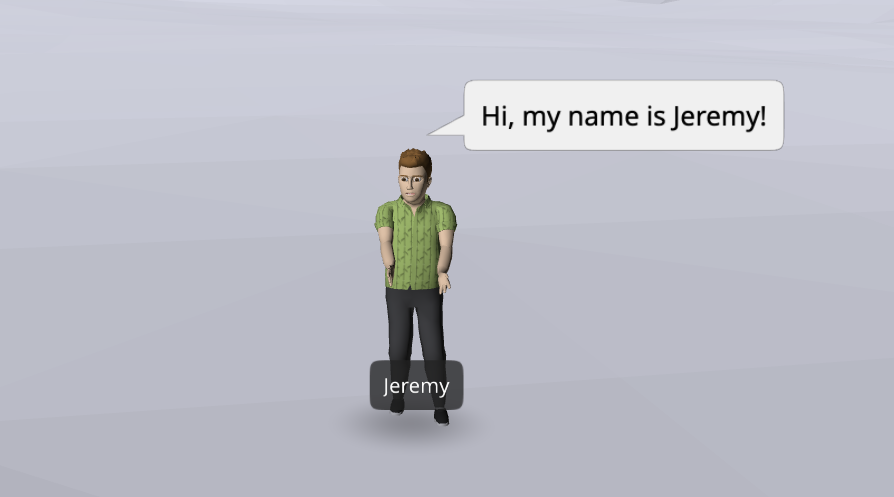
\includegraphics[width=0.55\textwidth]{./Images/Hello.png}
        \caption{Jeremy Says Hello}
    \end{figure}
    \begin{figure}[ht]
        \centering
        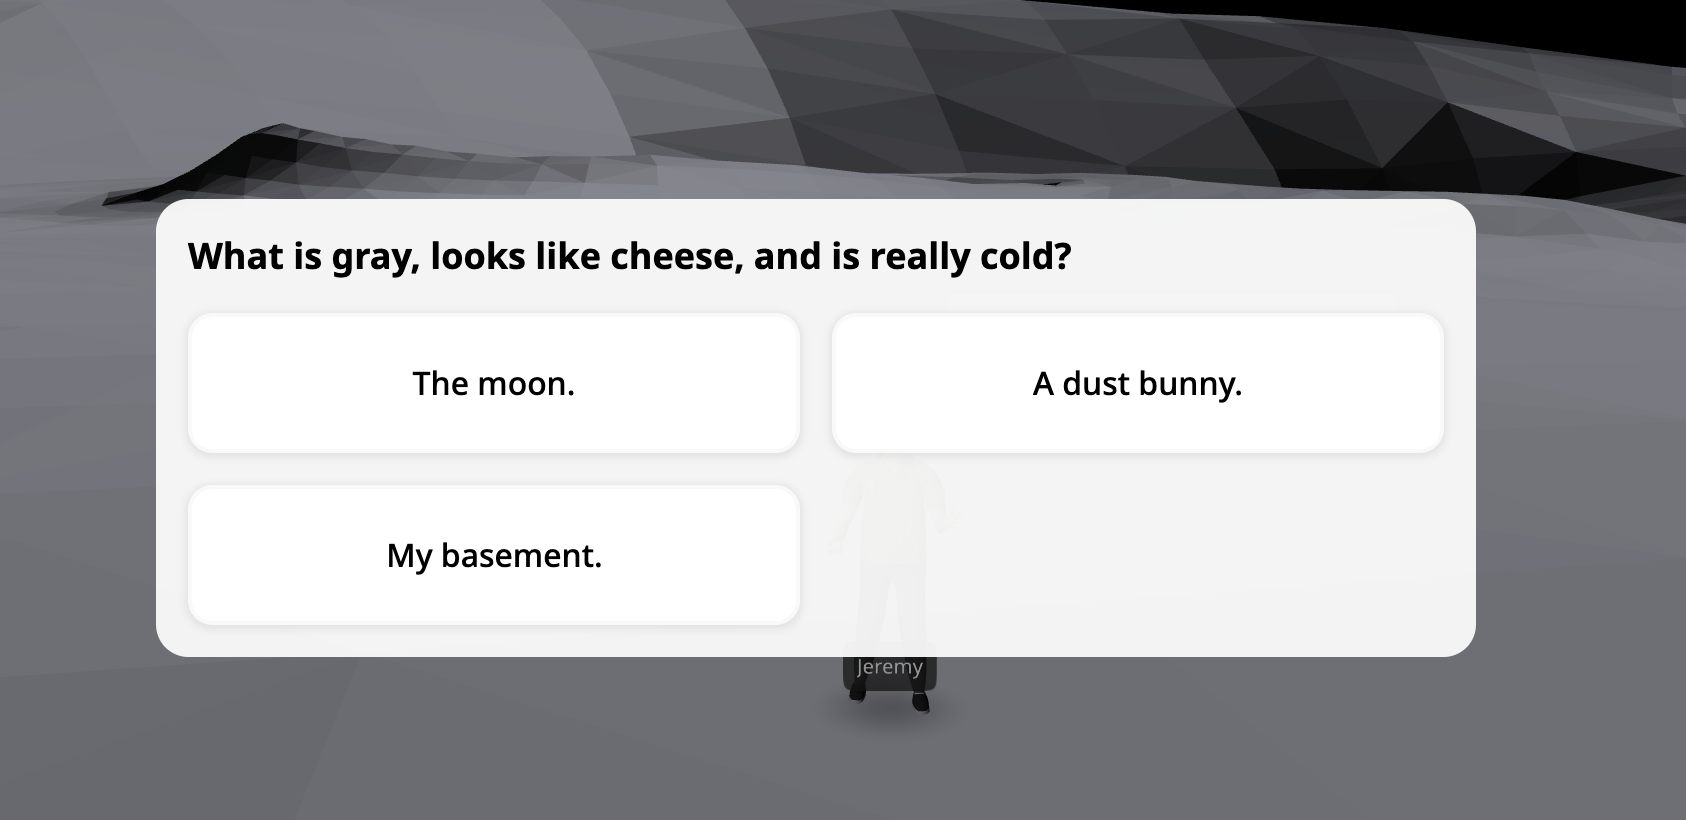
\includegraphics[width=0.55\textwidth]{./Images/First Riddle.png}
        \caption{First Riddle}
    \end{figure}
    \begin{figure}[ht]
        \centering
        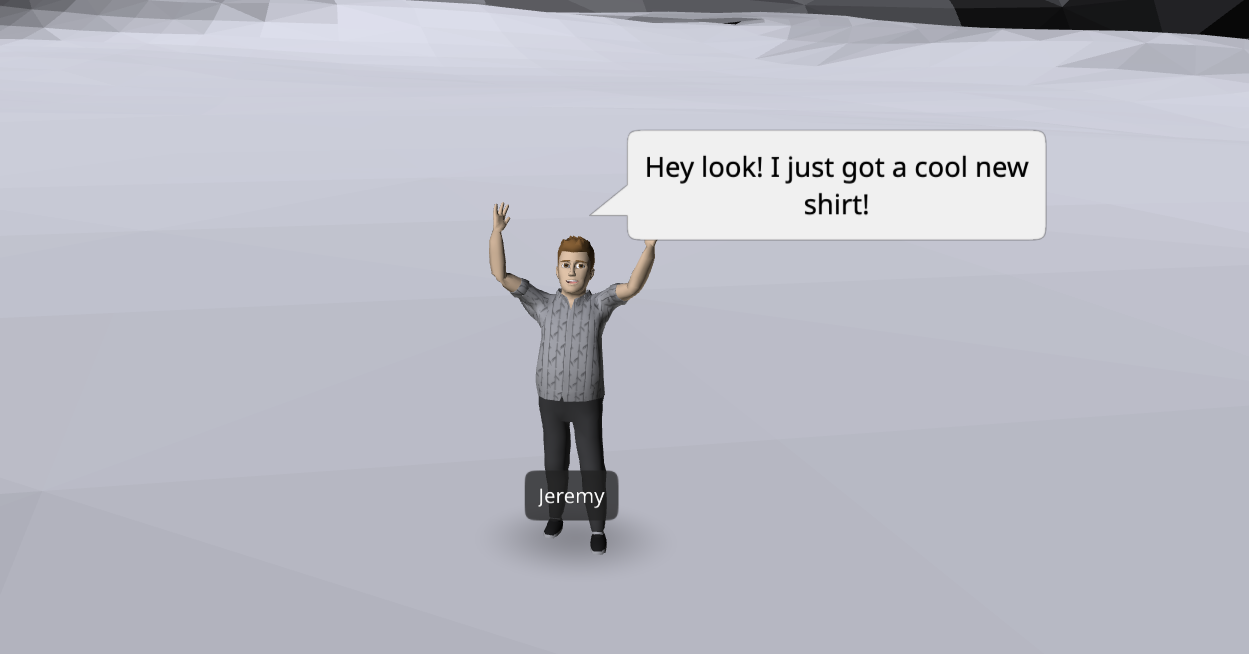
\includegraphics[width=0.55\textwidth]{./Images/Cool New Shirt.png}
        \caption{Cool New Shirt}
    \end{figure}
    \begin{figure}[ht]
        \centering
        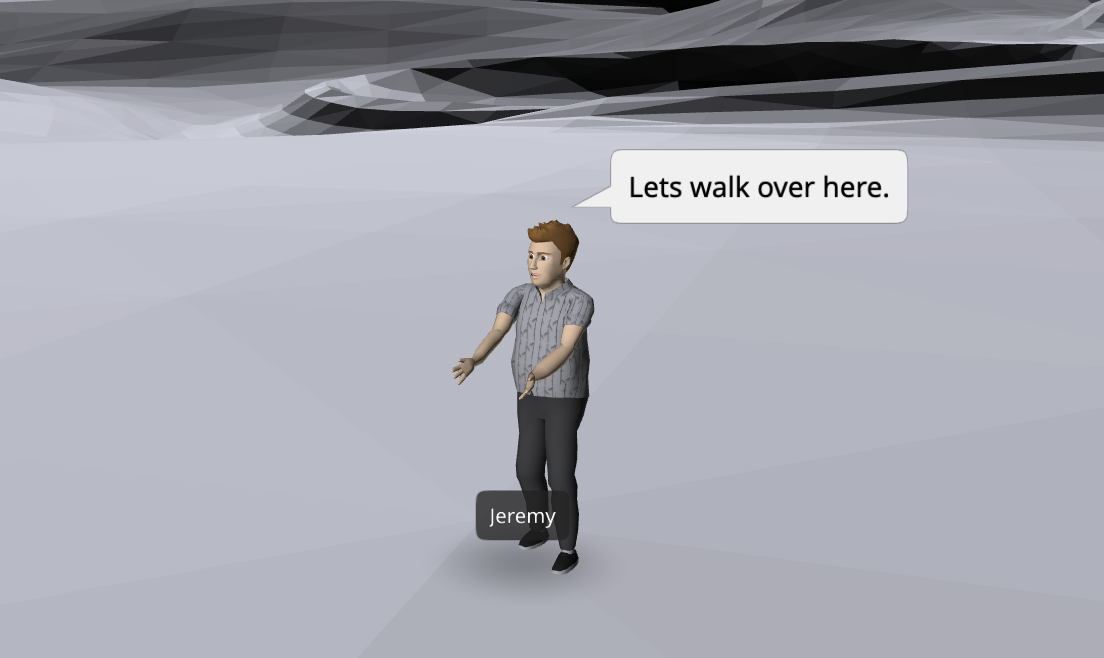
\includegraphics[width=0.55\textwidth]{./Images/Walking Over There.png}
        \caption{Jeremy Takes A Walk}
    \end{figure}
    \begin{figure}[ht]
        \centering
        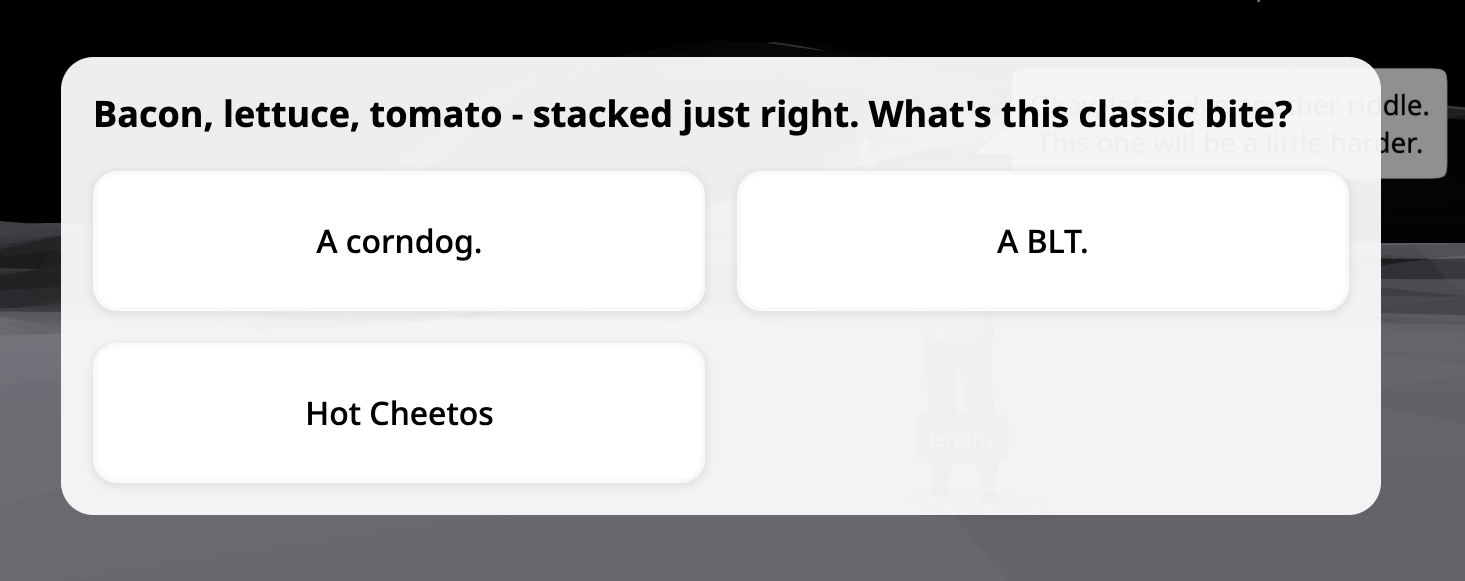
\includegraphics[width=0.55\textwidth]{./Images/Second Riddle.png}
        \caption{Second Riddle}
    \end{figure}
    \begin{figure}[ht]
        \centering
        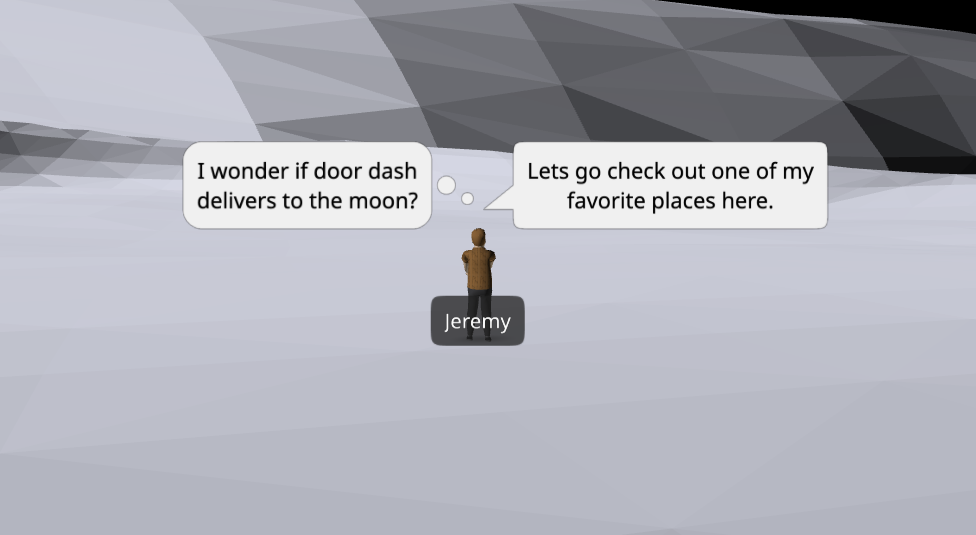
\includegraphics[width=0.55\textwidth]{./Images/Walking Away.png}
        \caption{Jeremy Walks Away}
    \end{figure}
    \clearpage
    \begin{figure}[ht]
        \centering
        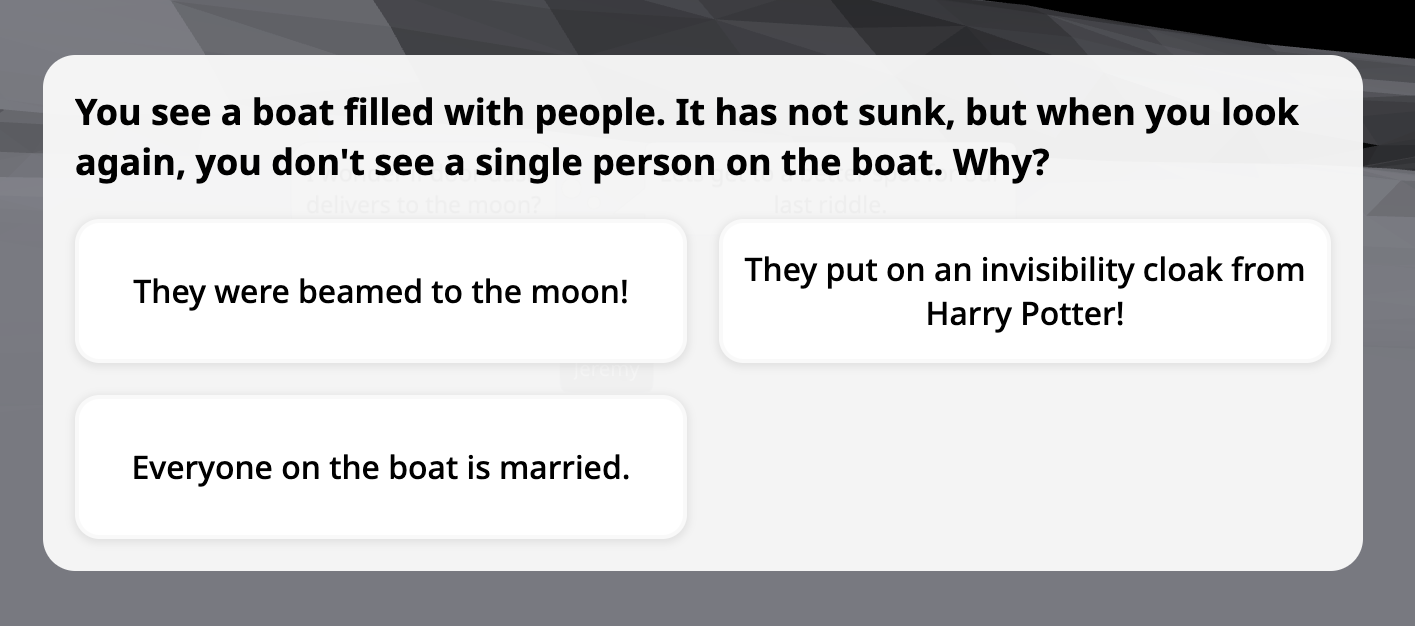
\includegraphics[width=0.55\textwidth]{./Images/Third Riddle.png}
        \caption{Third Riddle}
    \end{figure}
    \begin{figure}[ht]
        \centering
        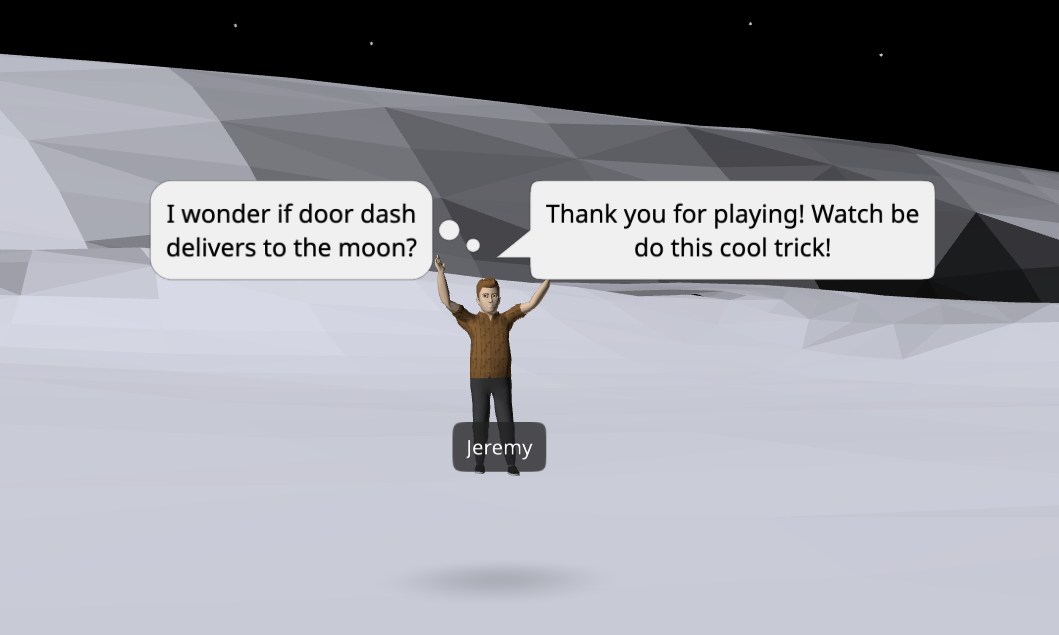
\includegraphics[width=0.55\textwidth]{./Images/Cool Trick.png}
        \caption{Jeremy's Cool Trick}
    \end{figure}
    \begin{figure}[ht]
        \centering
        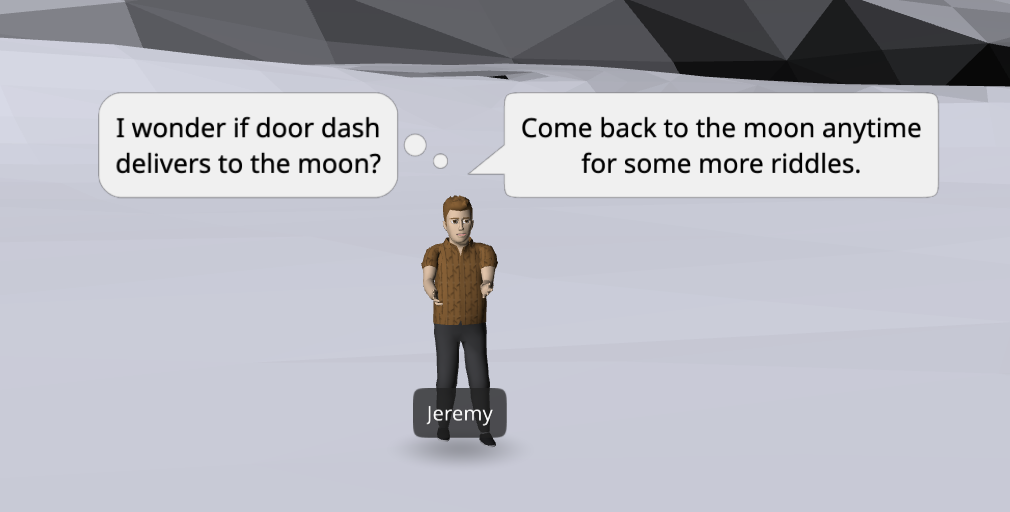
\includegraphics[width=0.55\textwidth]{./Images/Goodbye.png}
        \caption{Jeremy Says Goodbye}
    \end{figure}
\end{problem}